\documentclass{article}
\usepackage{tikz}
\usepackage{tikz-qtree}

\begin{document}

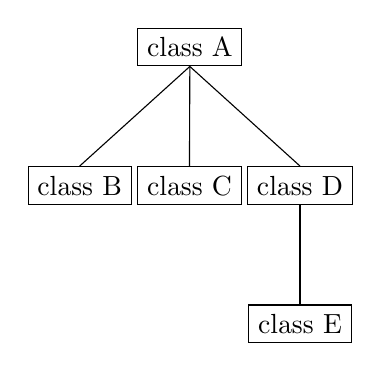
\begin{tikzpicture}
\tikzset{level distance=50pt}
\Tree [.\node[draw]{class A};
    [.\node[draw]{class B}; ]
    [.\node[draw]{class C}; ]
    [.\node[draw]{class D};
        \node[draw]{class E};
    ]
]
\end{tikzpicture}

\end{document}



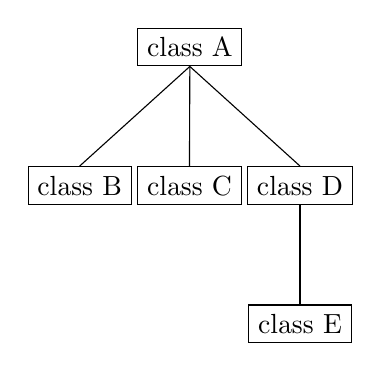
\begin{tikzpicture}
\tikzset{level distance=50pt}
\Tree
  [.\node[draw]{class A};
    [.\node[draw]{class B}; ]
    [.\node[draw]{class C}; ]
    [.\node[draw]{class D};
      \node[draw]{class E};
    ]
  ]
\end{tikzpicture}
